\section{Асимметричные протоколы}
\selectlanguage{russian}

Асимметричные протоколы, или же протоколы, основанные на криптосистемах с открытыми ключами, позволяют ослабить требования к предварительному этапу протоколов. Вместо общего секретного ключа, который должны иметь две стороны (либо обе стороны и доверенный центр), в рассматриваемых ниже протоколах стороны должны предварительно обменяться открытыми ключами (между собой либо между собой и доверенным центром). Такой предварительный обмен может проходить по открытому каналу связи, в предположении, что криптоаналитик не может повлиять на содержимое канала связи на данном этапе.

\subsection{Простой протокол}

Рассмотрим протокол распространения ключей с помощью асимметричных шифров. Введём обозначения: $K_B$ -- открытый ключ стороны $B$, а $K_A$ -- открытый ключ стороны $A$. Протокол включает три сеанса обмена информацией.
\begin{enumerate}
    \item В первом сеансе сторона $A$ посылает стороне $B$ сообщение:
            \[ A \rightarrow B: ~ E_{K_B}(K_1, A), \]
        где $K_1$ -- ключ, выработанный стороной $A$.
    \item Сторона $B$ получает $(K_1, A)$ и передаёт стороне $A$ наряду с другой информацией свой ключ $K_2$ в сообщении, зашифрованном с помощью открытого ключа $K_A$:
            \[ A \leftarrow B: ~ E_{K_A}(K_2, K_1, B). \]
    \item Сторона $A$ получает и расшифровывает сообщение $(K_2, K_1, B)$. Во время третьего сеанса сторона $A$, чтобы подтвердить, что она знает ключ $K_2$, посылает стороне $B$ сообщение:
            \[ A \rightarrow B: ~ E_{K_B}(K_2). \]
\end{enumerate}
Общий ключ формируется из двух ключей: $K_1$ и $K_2$.

\subsection{Протоколы с цифровыми подписями}

Существуют протоколы обмена, в которых перед началом обмена ключами генерируются подписи сторон $A$ и $B$, соответственно $S_A(m)$ и $S_B(m)$. В этих протоколах можно использовать различные одноразовые метки. Рассмотрим пример.
\begin{enumerate}
    \item Сторона $A$ выбирает ключ $K$ и вырабатывает сообщение:
            \[ \left( K, ~ t_A, ~ S_A(K, t_A, B) \right), \]
        где $t_A$ -- метка времени. Зашифрованное сообщение передаёт стороне $B$:
        \[ A \rightarrow B: ~ E_{K_B}(K, ~ t_A, ~ S_A(K, t_A, B)). \]
    \item Сторона $B$ получает это сообщение, расшифровывает $\left( K, ~ t_A, ~ S_A(K, t_A, B) \right)$ и вырабатывает свою метку времени $t_B$. Проверка считается успешной, если $|t_B - t_A | < \delta $. Сторона $B$ знает свои реквизиты и может осуществлять проверку подписи.
\end{enumerate}

Имеется второй вариант протокола, в котором шифрование и подпись выполняются раздельно.
\begin{enumerate}
    \item Сторона $A$ вырабатывает ключ $K$, использует одноразовую метку (или метку времени) $t_{A}$ и передаёт стороне $B$ два различных зашифрованных сообщения:
            \[ \begin{array}{ll}
                A \rightarrow B: & ~ E_{K_B}(K, t_A), \\
                A \rightarrow B: & ~ S_A(K, t_A, B). \\
            \end{array} \]
    \item Сторона $B$ получает это сообщение, расшифровывает $K, t_A$ и, добавив свои реквизиты, может проверить подпись $S_A(K, t_A, B)$.
\end{enumerate}

В третьем варианте протокола сначала производится шифрование, потом подпись.
\begin{enumerate}
    \item Сторона $A$ вырабатывает ключ $K$, использует одноразовую случайную метку или метку времени $t_A$ и передаёт стороне $B$ сообщение:
        \[ A \rightarrow B: ~ t_A, ~ E_{K_B}(K, A), ~ S_A(t_A, ~ K, ~ E_{K_B}(K, A)). \]
    \item Сторона $B$ получает это сообщение, расшифровывает $\left( K, ~ A \right)$ и проверяет подпись $S_A(t_A, ~ K, ~ E_{K_B}(K, A))$.
\end{enumerate}

\subsection{Протокол Диффи~---~Хеллмана}\index{протокол!Диффи~---~Хеллмана}
\selectlanguage{russian}

Алгоритм с открытым ключом впервые был предложен Диффи и Хеллманом в работе 1976 года <<Новые направления в криптографии>> (\langen{Bailey Whitfield Diffie, Martin Edward Hellman, ``New directions in cryptography''},~\cite{Diffie:Hellman:1976}).

Рассмотрим протокол Диффи~---~Хеллмана обмена информацией двух сторон $A$ и $B$. Задача состоит в том, чтобы создать общий сеансовый ключ.

Пусть $p$ -- большое простое число\index{число!простое}, $g$ -- примитивный элемент группы $\Z_p^*$, ~ $y = g^x \mod p$, причём $p,y,g$ известны заранее. Функцию $y=g^{x} \mod p$ считаем однонаправленной, то есть вычисление функции при известном значении аргумента является лёгкой задачей, а её обращение (нахождение аргумента) при известном значении функции -- трудной.

Протокол обмена состоит из следующих действий.
\begin{enumerate}
    \item Сторона $A$ выбирает случайное число $x: ~ 2 \leq x \leq p-1$, вычисляет и передаёт стороне $B$ сообщение:
        \[ A \rightarrow B: ~ g^x \mod p. \]
    \item Сторона $B$ выбирает случайное число $y: ~ 2\leq y \leq p-1$, вычисляет и передаёт стороне $A$:
        \[ A \leftarrow B: ~ g^y \mod p. \]
    \item Сторона $A$, используя известные ей значения $x$, $g^{y} \mod p$, вычисляет ключ:
        \[ K_{A} =(g^{y})^{x}\mod p=g^{xy} \mod p. \]
    \item Сторона $B$, используя известные ей значения $y$, $g^{x} \mod p$, вычисляет ключ:
        \[ K_{B} =(g^{x})^{y}\mod p=g^{xy}\mod p. \]
        В результате получаем равенство $K_A = K_B = K$.
\end{enumerate}

Таким способом создан общий секретный сеансовый ключ. В каждом новом сеансе используется этот же протокол для создания нового сеансового ключа.

Рассмотрим протокол Диффи~---~Хеллмана в ситуации, когда имеются три легальных пользователя $A,B,C$.

Каждая из сторон $A,B,C$ вырабатывает случайные числа $x,y,z$ соответственно и держит их в секрете.

\begin{enumerate}
    \item Первый этап обмена информацией аналогичен вышеописанному обмену информацией между двумя сторонами:
        \begin{enumerate}
            \item $A \rightarrow B: ~ g^x \mod p$.
            \item $B \rightarrow C: ~ g^y \mod p$.
            \item $C \rightarrow A: ~ g^z \mod p$.
        \end{enumerate}
    \item Второй этап состоит из передач сообщений:
        \begin{enumerate}
            \item $A \rightarrow B: ~ (g^z)^x = g^{zx} \mod p$.
            \item $B \rightarrow C: ~ (g^x)^y = g^{xy} \mod p$.
            \item $C \rightarrow A: ~ (g^y)^z = g^{yz} \mod p$.
        \end{enumerate}
    \item На завершающем третьем этапе стороны вычисляют:
        \begin{enumerate}
            \item $A: ~ K_A = (g^{yz})^x = g^{xyz} \mod p$.
            \item $B: ~ K_B = (g^{zx})^y = g^{xyz} \mod p$.
            \item $C: ~ K_C = (g^{xy})^z = g^{xyz} \mod p$.
        \end{enumerate}
\end{enumerate}

Как видно из произведённых действий, выработанные сторонами $A, B, C$ ключи совпадают: $K_A = K_B = K_C = K$. Следовательно, создан общий секретный сеансовый ключ $K$ для трёх участников.

Таким же образом можно построить протокол Диффи~---~Хеллмана для любого числа легальных пользователей.

Рассмотрим этот двусторонний протокол с точки зрения криптоаналитика, желающего узнать ключ $K$. Предположим, ему удалось перехватить сообщения $g^{x}\mod p$ и $g^{y}\mod p $. Используя заранее известные данные $g,p $ и эти сообщения, криптоаналитик старается найти хотя бы одно из чисел $(x,y)$, то есть решить задачу дискретного логарифма. В настоящее время эта задача считается вычислительно трудной при обычно выбираемых значениях $p\sim 2^{1024}$.

Существует атака активного криптоаналитика\index{криптоаналитик!активный}, названная <<человек посередине>> (man-in-the-middle)\index{атака!<<человек посередине>>}. Пусть имеются две легальные стороны $A$ и $B$ и нелегальная сторона $E$ -- активный криптоаналитик\index{криптоаналитик!активный}, который имеет возможность перехватывать и подменять сообщения как от $A$, так и от $B$:
    \[ A \leftrightsquigarrow E \leftrightsquigarrow B. \]
    %\[ A \leftrightarrow E \leftrightarrow B. \]

\begin{enumerate}
    \item Подмена ключей.
        \begin{enumerate}
            \item Сторона $A$ передаёт стороне $B$ сообщение:
                \[ A \overset{E}{\nrightarrow} B: ~ g^x \mod p. \]
            \item Сторона $E$ перехватывает сообщение $g^x \mod p$, сохраняет его и, зная $g$, передаёт стороне $B$ своё сообщение:
                \[ E \rightarrow B: ~ g^z \mod p. \]
            \item Сторона $B$ передаёт стороне $A$ сообщение:
                \[ A \overset{E}{\nleftarrow} B: ~ g^y \mod p. \]
            \item Сторона $E$ перехватывает сообщение $g^y \mod p$, сохраняет его и передаёт стороне $A$ своё сообщение:
                \[ A \leftarrow E: ~ g^z \mod p \]
                или какое-то другое.
            \item Таким образом, между сторонами $A$ и $E$ образуется общий секретный ключ $K_{AE}$, между $B$ и $E$ -- ключ $K_{BE}$, причём $A$ и $B$ не знают, что у них ключи со стороной $E$, а не друг с другом:
                \[ \begin{array} {l}
                    K_{AE} = g^{xz} \mod p, \\
                    K_{BE} = g^{yz} \mod p. \\
                \end{array} \]

        \end{enumerate}
    \item Подмена сообщений.
        \begin{enumerate}
            \item Сторона $A$ посылает $B$ сообщение $m$, зашифрованное на ключе $K_{AE}$:
                % \rightsquigarrow
                \[ A \overset{E}{\nrightarrow} B: ~ E_{K_{AE}}(m). \]
            \item Сторона $E$ перехватывает сообщение, расшифровывает с ключом $K_{AE}$, возможно, подменяет на $m'$, зашифровывает с ключом $K_{BE}$ и посылает $B$:
                \[ E \rightarrow B: ~ E_{K_{BE}}(m'). \]
            \item То же самое происходит при обратной передаче от $B$ к $A$.
        \end{enumerate}
\end{enumerate}

Криптоаналитик $E$ имеет возможность перехватывать и подменять все передаваемые сообщения. Если по тексту письма нельзя обнаружить участие криптоаналитика в обмене информацией, то атака <<человек посередине>>\index{атака!<<человек посередине>>} успешна.

Существует несколько протоколов для защиты от атаки этого типа.


%\section{Протоколы с аутентификацией}

\subsection{Односторонняя аутентификация}

\textbf{Протокол Эль-Гамаля}\index{протокол!Эль-Гамаля} относится к протоколам с аутентификацией одного из двух легальных пользователей.
\selectlanguage{russian}
\begin{enumerate}
    \item Для начала стороны выбирают общие параметры $p, g$, где $p$ -- большое простое число, а $g$ -- примитивный элемент поля $\Z_p^*$.
    \item Сторона $B$ создаёт свои закрытый и открытый ключи:
            \[ \SK_B = b, ~ \PK_B = g^b \mod p, \]
        $b$ -- случайное секретное число, $2 \leq b \leq p-1$.

        Открытый ключ $\PK_B$ находится в общем открытом доступе для всех сторон, поэтому криптоаналитик $E$ не может подменить его -- подмена будет заметна.
    \item Сторона $A$ вырабатывает свой секрет $x$, сеансовый ключ
            \[ K_A = (\PK_B)^x = g^{bx} \mod p \]
        и отправляет $B$:
            \[ A \rightarrow B: ~ g^x \mod p. \]
    \item Сторона $B$, получив от $A$ число $g^x \mod p$, использует его и свой секрет $\SK_B = b$, чтобы создать свой ключ
            \[ K_B = (g^x)^{\SK_B} = g^{bx} \mod p, \]
        то есть сеансовые ключи обеих сторон совпадают:
            \[ K_A = K_B = K. \]
\end{enumerate}

Достоинством этого протокола является следующее его свойство. Если ключи $K_A$ и $K_B$ совпали и стороны могут обмениваться информацией, то сторона $A$ аутентифицирует сторону $B$, так как для шифрования она использовала открытый ключ $B$, который не может быть незаметно подменён, и только сторона $B$ может расшифровывать сообщения.

Что касается криптоаналитика в качестве <<человека посередине>>, то он может отправлять ложные сообщения, но не может узнать ключ $K$ и читать сообщения.

Есть протоколы, в которых стороны, осуществляющие обмен информацией, являются равноправными. Они называются протоколами взаимной аутентификации.


\subsection{Взаимная аутентификация шифрованием}
\selectlanguage{russian}

К протоколам взаимной аутентификации принадлежит семейство протоколов, разработанных Ц.~Мацумото (\langen{Tsutomu Matsumoto}), И.~Такашима (\langen{Youichi Takashima}) и Х.~Имаи (\langen{Hideki Imai}) и названных по первым буквам фамилий авторов -- \emph{протоколы MTI}\index{протоколы!MTI}.

Здесь к открытым данным относятся:
    \[ p, ~~ g, ~~ \PK_A = g^a \mod p, ~~ \PK_B = g^b \mod p. \]
Каждый из пользователей $A$ и $B$ обладает парой долговременных ключей для \emph{схемы шифрования с открытым ключом}: закрытым ключом расшифрования $\SK$ и открытым ключом шифрования $\PK$.
\[ \begin{array}{ll}
    A: & ~ \SK_A = a, ~~ \PK_A = g^a \mod p, \\
    B: & ~ \SK_B = b, ~~ \PK_B = g^b \mod p. \\
\end{array} \]

\textbf{Протокол MTI}:
\begin{enumerate}
    \item Сторона $A$ генерирует случайное число $x, ~ 2\leq x\leq p-1$, создаёт и отправляет $B$ сообщение:
        \[ A \rightarrow B: ~ g^x \mod p. \]
    \item Сторона $B$ генерирует случайное число $y, ~ 2\leq y\leq p-1$, создаёт и отправляет $A$ сообщение:
        \[ A \leftarrow B: ~ g^y \mod p. \]
    \item Сторона $A$, используя открытые данные и полученное сообщение, создаёт сеансовый ключ:
        \[ K_A = (g^b)^x \cdot (g^y)^a = g^{bx+ay} \mod p. \]
    \item Сторона $B$, используя открытые данные и полученное сообщение, создаёт сеансовый ключ:
        \[ K_B = (g^x)^b \cdot (g^a)^y = g^{bx+ay} \mod p. \]
        Сеансовые ключи обеих сторон совпадают:
        \[ K_{A} =K_{B} = K. \]
\end{enumerate}

В описанном протоколе, как и в протоколе Эль-Гамаля\index{криптосистема!Эль-Гамаля}, происходит взаимная аутентификация сторон: открытые ключи сторон незаметно подменить невозможно. Наблюдая сообщения протокола, вычислить $g^{bx+ay}$ можно, только если известны значения $a,x$ или $b,y$, что представляет собой задачу дискретного логарифмирования, вычислительно трудную на сегодняшний день.


\subsection{Взаимная аутентификация схемой ЭП}
\selectlanguage{russian}

\emph{Протокол STS (Station-to-Station)}\index{протокол!Station-to-Station} предназначен для систем мобильной связи. Он использует идеи протокола Диффи~---~Хеллмана\index{протокол!Диффи~---~Хеллмана} и криптосистемы RSA\index{криптосистема!RSA}. Особенностью протокола является использование механизма электронной подписи\index{электронная подпись} для взаимной аутентификации сторон\index{аутентификация!взаимная}.

Здесь открытые общедоступные данные:
    \[ p, ~ g, ~ \PK_A, ~ \PK_B. \]

Каждая из сторон $A$ и $B$ обладает долговременной парой ключей: закрытым ключом для создания электронной подписи $\SK$ и открытым ключом для проверки подписи $\PK$:
\[ \begin{array}{ll}
    A: & ~ \SK_A, ~~ \PK_A, \\
    B: & ~ \SK_B, ~~ \PK_B. \\
\end{array} \]

Протокол состоит из трёх раундов обмена информацией между сторонами $A$ и $B$.
\begin{enumerate}
    \item Сторона $A$ создаёт секретное случайное число $x: 2 \leq x \leq p-1$ и отправляет $B$:
            \[ A \rightarrow B: ~ g^x \mod p. \]
    \item Сторона $B$ создаёт секретное случайное число $y: 2 \leq y \leq p-1$, вычисляет общий секретный ключ
            \[ K = (g^x)^y = g^{xy} \mod p, \]
        с помощью которого создаёт шифрованное сообщение $E_K(S_B(g^x, g^y))$ для аутентификации, и отправляет $A$:
            \[ A \leftarrow B: ~ \left( g^y \mod p, ~~ E_K( S_B( g^x, g^y)) \right). \]
    \item Сторона $A$ с помощью $x$, $g^y \mod p$ вычисляет общий секретный ключ
            \[ K = (g^y)^x \mod p = g^{xy} \mod p \]
        и расшифровывает сообщение:
            \[ D_K( E_K( S_B( g^x, g^y))) = S_B( g^x, g^y). \]
            Затем аутентифицирует сторону $B$, проверяя подпись $S_B$ открытым ключом $\PK_B$. Вычисляет и пересылает стороне $B$ сообщение:
            \[ A \rightarrow B: ~ E_K( S_A( g^x, g^y)). \]
    \item Сторона $B$ расшифровывает принятое сообщение:
            \[ D_K( E_K( S_A( g^x, g^y))) = S_A( g^x, g^y) \]
        и осуществляет аутентификацию, выполняя проверку подписи $S_A$ с помощью открытого ключа $\PK_A$.
\end{enumerate}


\subsection{Взаимная аутентификация с доверенным центром}
\selectlanguage{russian}

В \emph{протоколе Жиро}\index{протокол!Жиро} (\langfr{Marc Girault},~\cite{Girault:1990, Girault:1991}) участвуют три стороны -- $A$, $B$ и надёжный центр $T$.
\begin{enumerate}
    \item У стороны $T$ есть открытый и закрытый ключи криптосистемы RSA\index{криптосистема!RSA},
        \[ n=pq, ~ e, ~ d=e^{-1} \mod \varphi(n), \]
        с дополнительным параметром $g$ -- генератором подгруппы максимально возможного порядка мультипликативной группы $\Z_n^*$:
        \[ \begin{array}{l}
            \PK_T = (n, e, g) ~~\text{открытый ключ}, \\
            \SK_T = (d) ~~ \text{закрытый ключ}. \\
        \end{array} \]
    \item Стороны $A$ и $B$ независимо друг от друга создают свои открытые и закрытые ключи, обмениваясь информацией с центром $T$ по надёжному защищённому каналу. Стороны $A$ и $B$ выбирают свои закрытые ключи:
        \[ \begin{array}{l}
            \SK_A = a, \\
            \SK_B = b \\
        \end{array} \]
     и отправляют центру сообщения:
        \[ \begin{array}{ll}
            A \to T: & ~ I_A, ~~ g^{-\SK_A} = g^{-a} \mod n, \\
            B \to T: & ~ I_B, ~~ g^{-\SK_B} = g^{-b} \mod n, \\
        \end{array} \]
        где $I_A, I_B$ -- числовые идентификаторы сторон.
    \item Центр $T$ вычисляет открытые ключи для $A$ и $B$ и также по надёжному каналу передаёт им:
        \[ \begin{array}{ll}
            A \leftarrow T: & ~ \PK_A = (g^{-\SK_A} - I_A)^{\SK_T} = (g^{-a} - I_A)^d \mod n, \\
            B \leftarrow T: & ~ \PK_B = (g^{-\SK_B} - I_B)^{\SK_T} = (g^{-b} - I_B)^d \mod n. \\
        \end{array} \]
    \item Теперь стороны $A$ и $B$ могут создать общий секретный симметричный сеансовый ключ. Например, $A$ находит:
        \[ \begin{array}{ll}
            A: ~~ K_A & = ~ (\PK_B^e + I_B)^{\SK_A} ~ = \\
                & = ~ (((g^{-b} - I_B)^d)^e + I_B)^a ~ = \\
                & = ~ (g^{-b} - I_B + I_B)^a ~ = \\
                & = ~ g^{-ab} \mod n. \\
        \end{array} \]
        Аналогично $B$ вычисляет:
            \[ K_B = (\PK_A^e + I_A)^{\SK_B} = g^{-ab} \mod n. \]
        Как видно, ключи одинаковы:
            \[ K = K_A = K_B = g^{-ab} \mod n. \]
\end{enumerate}


\subsection{Схема Блома}\label{section-bloms-scheme}\index{схема!Блома|(}
\selectlanguage{russian}

Схема Блома (\langen{Rolf Blom},~\cite{Blom:1984, Blom:1985}) используется в протоколе HDCP\index{протокол!HDCP} (\langen{High-bandwidth Digital Content Protection}) для предотвращения копирования высококачественного видеосигнала. Предполагается, что некоторый доверенный центр распределит ключи таким образом, что легальные производители видеокарт, мониторов высокого разрешения и других компонент будут передавать видеоконтент по защищённому каналу, а <<пиратские>> устройства не смогут эти данные перехватить, и, например, записать на другой носитель.

На этапе инициализации доверенный центр выбирает симметричную матрицу $D_{m,m}$ над конечным полем $\GF p$. Для присоединения к сети распространения ключей, новый участник либо самостоятельно, либо с помощью доверенного центра выбирает новый открытый ключ (идентификатор) $I_i$, представляющий собой вектор длины $m$ над $\GF p$. Доверенный центр вычисляет для нового участника закрытый ключ $K_i$:
\begin{equation}
	K_i = D_{m,m} I_i.
	\label{eq:blom_center_matrix}
\end{equation}

Симметричность матрицы $D_{m,m}$ доверенного центра позволяет любым двум участникам сети создать общий сеансовый ключ. Пусть Алиса и Боб -- легальные пользователи сети, то есть они обладают открытыми ключами $I_A$ и $I_B$ соответственно, а их закрытые ключи $K_A$ и $K_B$ были вычислены одним и тем же доверенным центром по формуле~\ref{eq:blom_center_matrix}. Тогда протокол выработки общего секретного ключа выглядит следующим образом (рис.~\ref{fig:key_distribution-bloms-scheme}).

\begin{figure}
    \centering
    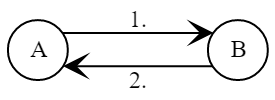
\includegraphics[width=0.5\textwidth]{pic/key_distribution-bloms-scheme}
    \caption{Взаимодействие участников в схеме Блома\label{fig:key_distribution-bloms-scheme}}
\end{figure}

\begin{protocol}
    \item[(1)] $Alice \to \left\{ I_A \right\} \to Bob$
    \item[(2)] Боб вычисляет $K_{BA} = K^T_B I_A = I^T_B D_{m,m} I_A$.
    \item[{}] $Bob \to \left\{ I_B \right\} \to Alice$
    \item[(3)] Алиса вычисляет $K_{AB} = K^T_A I_B = I^T_A D_{m,m} I_B$.
\end{protocol}

Из симметричности матрицы $D_{m,m}$ следует, что значения $K_{AB}$ и $K_{BA}$ совпадут, они же и будут являться общим секретным ключом для Алисы и Боба. Этот секретный ключ будет свой для каждой пары легальных пользователей сети.

Присоединение новых участников к схеме строго контролируется доверенным центром, что позволяет защитить сеть от нелегальных пользователей. Надёжность данной схемы основывается на невозможности восстановить исходную матрицу. Однако для восстановления матрицы доверенного центра размера $m \times m$ необходимо и достаточно всего $m$ пар линейно независимых открытых и закрытых ключей. В 2010-м году компания Intel, которая является <<доверенным центром>> для пользователей системы защиты HDCP, подтвердила, что криптоаналитикам удалось найти секретную матрицу (точнее, аналогичную ей), используемую для генерации ключей в упомянутой системе предотвращения копирования высококачественного видеосигнала.

\index{схема!Блома|)}
